\documentclass[11pt,a4paper]{article}
\usepackage[margin=18mm]{geometry}
\usepackage{amsmath,amssymb,mathtools}
\usepackage{booktabs,array,enumitem}
\usepackage[dvipsnames]{xcolor}
\usepackage{graphicx,listings,tikz,float,needspace}
\usetikzlibrary{arrows.meta,positioning}
\usepackage[most]{tcolorbox}
\usepackage{hyperref}
\hypersetup{colorlinks=true,urlcolor=MidnightBlue,linkcolor=MidnightBlue}
\setlength{\parindent}{0pt}\setlength{\parskip}{4pt}
\newcommand{\course}{PHY4605 Computational Methods in Physics}
\newcommand{\units}[1]{\,\mathrm{#1}}
\newtcolorbox{keybox}{colback=RoyalBlue!5,colframe=RoyalBlue!65!black,boxrule=.7pt,arc=2mm}
\newtcolorbox{checkbox}{colback=ForestGreen!5,colframe=ForestGreen!55!black,boxrule=.7pt,arc=2mm}
\newtcolorbox{aibox}{colback=BurntOrange!7,colframe=BurntOrange!80!black,boxrule=.7pt,arc=2mm}
\lstdefinestyle{matlabstyle}{language=Matlab,basicstyle=\ttfamily\footnotesize,keywordstyle=\color{RoyalBlue!75!black},commentstyle=\color{ForestGreen!55!black},stringstyle=\color{BurntOrange!80!black},numbers=left,numberstyle=\scriptsize\color{black!50},numbersep=5pt,frame=single,rulecolor=\color{RoyalBlue!25},backgroundcolor=\color{RoyalBlue!3},showstringspaces=false,columns=fullflexible,keepspaces=true,breaklines=true}
\begin{document}
{\large\textsc{\course}}\\[-2pt]
{\small Learning Note \textbar\ Week 3}\par\vspace{4pt}
{\LARGE\bfseries Two-by-Two Linear Systems through Kirchhoff Circuits}\par\vspace{3pt}
\textit{Turn two familiar circuit equations into a small linear system that can be solved, checked, and interpreted.}

\begin{keybox}\textbf{Physical question.} Two resistor loops share one resistor. If the source voltages and resistances are known, how can we find the two loop currents without losing track of signs, units, or physical meaning?\end{keybox}

\section*{Core learning outcomes}
\begin{enumerate}[nosep,leftmargin=5mm]
\item derive two consistent Kirchhoff equations from a stated current convention;
\item map those equations to $A\mathbf{x}=\mathbf{b}$ and solve them with MATLAB backslash; and
\item validate the solution by direct substitution and interpret the current signs physically.
\end{enumerate}

\section*{1. Start from the circuit, not the matrix}
Choose both mesh currents clockwise. Let the left private resistor be $R_1=2\units{\Omega}$, the right private resistor $R_2=3\units{\Omega}$, and the shared resistor $R_s=1\units{\Omega}$. The source rises are $V_1=5\units{V}$ and $V_2=2\units{V}$. The battery polarities below make those rises explicit: the long plate is positive, so the left source is traversed upward and the right source downward by the clockwise mesh currents.

\begin{center}
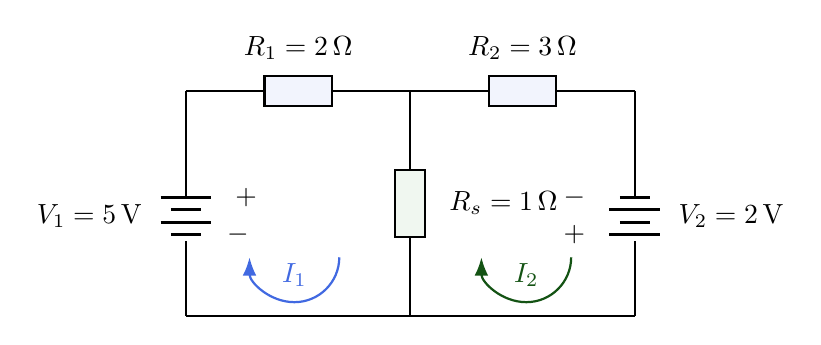
\begin{tikzpicture}[>=Latex,thick,scale=0.95]
% Left battery: positive terminal at the top, so the clockwise traversal is a rise.
\draw (0,0)--(3,0) (0,0)--(0,1.00);
\draw[line width=1.1pt] (-0.20,1.08)--(0.20,1.08);
\draw[line width=1.1pt] (-0.34,1.24)--(0.34,1.24);
\draw[line width=1.1pt] (-0.20,1.42)--(0.20,1.42);
\draw[line width=1.1pt] (-0.34,1.58)--(0.34,1.58);
\draw (0,1.58)--(0,3) (0,3)--(1.05,3);
\draw[fill=RoyalBlue!7] (1.05,2.80) rectangle (1.95,3.20);
\draw (1.95,3)--(3,3);
\draw (3,0)--(6,0) (6,0)--(6,1.00);
% Right battery: positive terminal at the bottom, so the clockwise traversal is a rise.
\draw[line width=1.1pt] (5.66,1.08)--(6.34,1.08);
\draw[line width=1.1pt] (5.80,1.24)--(6.20,1.24);
\draw[line width=1.1pt] (5.66,1.42)--(6.34,1.42);
\draw[line width=1.1pt] (5.80,1.58)--(6.20,1.58);
\draw (6,1.58)--(6,3) (3,3)--(4.05,3);
\draw[fill=RoyalBlue!7] (4.05,2.80) rectangle (4.95,3.20);
\draw (4.95,3)--(6,3);
\draw (3,0)--(3,1.05);
\draw[fill=ForestGreen!7] (2.80,1.05) rectangle (3.20,1.95);
\draw (3,1.95)--(3,3);
\draw (1.5,3.28) node[above] {$R_1=2\,\Omega$};
\draw (4.5,3.28) node[above] {$R_2=3\,\Omega$};
\draw (3.20,1.5) node[right=5pt] {$R_s=1\,\Omega$};
\draw (-0.45,1.33) node[left] {$V_1=5\,\mathrm{V}$};
\draw (0.45,1.58) node[right=2pt] {$+$};
\draw (0.34,1.08) node[right=2pt] {$-$};
\draw (6.45,1.33) node[right] {$V_2=2\,\mathrm{V}$};
\draw (5.55,1.08) node[left=2pt] {$+$};
\draw (5.55,1.58) node[left=2pt] {$-$};
% Keep the clockwise mesh arrows in the open lower half of each loop.
\draw[->,RoyalBlue] (2.05,0.78) arc[start angle=0,end angle=-180,radius=0.60] node[midway,above=2pt] {$I_1$};
\draw[->,ForestGreen!60!black] (5.15,0.78) arc[start angle=0,end angle=-180,radius=0.60] node[midway,above=2pt] {$I_2$};
\end{tikzpicture}
\end{center}

Across the shared resistor, the two mesh currents oppose each other. If we define the shared-branch direction to follow mesh 1, then
\[
I_{\mathrm{shared}}=I_1-I_2.
\]

\begin{checkbox}\textbf{Prediction checkpoint.} Both chosen mesh-current directions should give positive currents. The larger source and smaller private resistance suggest $I_1>I_2$.\end{checkbox}

\section*{2. Write Kirchhoff equations in words first}
For the left loop: \emph{left private voltage drop plus shared-resistor voltage drop equals the left source rise}. Therefore
\[
R_1I_1+R_s(I_1-I_2)=V_1,
\]
or
\[
(R_1+R_s)I_1-R_sI_2=V_1.
\]

For the right loop, the shared-resistor contribution is reversed:
\[
-R_sI_1+(R_2+R_s)I_2=V_2.
\]

Every term has units of volts because $\Omega\times\mathrm{A}=\mathrm{V}$.

\section*{3. Map each equation to one matrix row}
The two equations become
\[
\begin{bmatrix}
R_1+R_s & -R_s\\
-R_s & R_2+R_s
\end{bmatrix}
\begin{bmatrix}I_1\\I_2\end{bmatrix}
=
\begin{bmatrix}V_1\\V_2\end{bmatrix}.
\]
With the locked values,
\[
\underbrace{\begin{bmatrix}3&-1\\-1&4\end{bmatrix}}_{A\;(\Omega)}
\underbrace{\begin{bmatrix}I_1\\I_2\end{bmatrix}}_{\mathbf{x}\;(\mathrm A)}
=
\underbrace{\begin{bmatrix}5\\2\end{bmatrix}}_{\mathbf b\;(\mathrm V)}.
\]

\begin{keybox}\textbf{Key idea.} A matrix is only a compact storage format for the two physical equations. Every coefficient must be traceable back to one Kirchhoff term.\end{keybox}

\section*{4. Audit the matrix before solving}
Before asking MATLAB for a solution, read the matrix back as physics. The safest habit is to point to one entry at a time and ask: \emph{which unknown does this multiply, which loop equation does it belong to, and why does it have this sign?}

\begin{center}
\small
\begin{tabular}{>{\raggedright\arraybackslash}p{.15\linewidth}>{\centering\arraybackslash}p{.15\linewidth}>{\raggedright\arraybackslash}p{.54\linewidth}}
\toprule
\textbf{Entry} & \textbf{Value} & \textbf{Physical origin}\\
\midrule
$A_{11}$ & $3\,\Omega$ & $R_1+R_s$: resistance multiplying $I_1$ in the left-loop equation\\
$A_{12}$ & $-1\,\Omega$ & $-R_s$: effect of $I_2$ on the shared-resistor drop in the left loop\\
$A_{21}$ & $-1\,\Omega$ & $-R_s$: effect of $I_1$ on the shared-resistor drop in the right loop\\
$A_{22}$ & $4\,\Omega$ & $R_2+R_s$: resistance multiplying $I_2$ in the right-loop equation\\
\bottomrule
\end{tabular}
\end{center}

The diagonal terms are positive sums because each mesh current passes through its own private resistor and the shared resistor. The off-diagonal terms are negative because the other mesh current opposes the chosen current through the shared resistor. The source vector is $\mathbf b=[5\;2]^T\mathrm V$. This sign pattern comes from the chosen arrows, not from a matrix rule to memorise.

\begin{checkbox}\textbf{Units audit.} Row 1 reads $(3\,\Omega)I_1+(-1\,\Omega)I_2=5\,\mathrm V$. Both terms on the left are voltages. Row 2 has the same dimensional structure. If one coefficient were accidentally entered in volts or amperes instead of ohms, the matrix multiplication would no longer represent Kirchhoff's voltage law even if MATLAB still accepted the numbers.\end{checkbox}

\subsection*{A quick coefficient-tracing routine}
Before solving, ask three questions for any entry: \emph{which physical equation is this row, which unknown is this column, and why does this coefficient have this sign and unit?} For example, $A_{12}=-1\,\Omega$ means that the coefficient multiplying $I_2$ in the left-loop equation is $-R_s$.

\begin{keybox}\textbf{Representation checkpoint.} Cover the equations above and use only the matrix to reconstruct the left-loop equation. Then cover the matrix and rebuild its first row from the left-loop equation. You should be able to move in both directions.\end{keybox}

\section*{5. Pseudocode before MATLAB}
\begin{enumerate}[nosep,leftmargin=7mm]
\item store the resistances and source voltages;
\item build one matrix row from each Kirchhoff equation;
\item store the two source voltages in a column vector;
\item solve the two unknown currents;
\item reconstruct the shared-branch current;
\item substitute the currents back into both original equations; and
\item interpret the current signs and magnitudes.
\end{enumerate}

\section*{6. Solve the supplied system in MATLAB}
\begin{lstlisting}[style=matlabstyle]
R1_ohm = 2; R2_ohm = 3; Rs_ohm = 1;
V1_V = 5; V2_V = 2;
A_ohm = [R1_ohm+Rs_ohm, -Rs_ohm; ...
         -Rs_ohm, R2_ohm+Rs_ohm];
b_V = [V1_V; V2_V];
x_A = A_ohm\b_V;
I1_A = x_A(1);
I2_A = x_A(2);
\end{lstlisting}

The solution is $I_1=2\units{A}$ and $I_2=1\units{A}$. The reconstructed shared-branch current is
\[
I_{\mathrm{shared}}=2-1=1\units{A}.
\]

\section*{7. Core validation: substitute into the original equations}
For the left equation,
\[
3(2)-1(1)=5\units{V},
\]
which reproduces the 5 V source. For the right equation,
\[
-1(2)+4(1)=2\units{V},
\]
which reproduces the 2 V source.

\begin{lstlisting}[style=matlabstyle]
left_V = (R1_ohm+Rs_ohm)*I1_A - Rs_ohm*I2_A;
right_V = -Rs_ohm*I1_A + (R2_ohm+Rs_ohm)*I2_A;
check_V = [left_V-V1_V; right_V-V2_V];
assert(max(abs(check_V)) < 1e-12)
\end{lstlisting}

\begin{checkbox}\textbf{Validation result.} Both reconstructed loop voltages match the original sources. This directly checks the equations that represent the circuit.\end{checkbox}

\section*{8. Read the numerical solution back into the circuit}
Both currents are positive, so the actual mesh currents follow the assumed clockwise arrows. If MATLAB had returned a negative value, that would not automatically mean the calculation failed; it would mean the actual current runs opposite to the arrow chosen before solving.

The two numbers also tell us something about the shared branch. Because $I_1=2\units{A}$ and $I_2=1\units{A}$ act in opposite directions through $R_s$,
\[
I_{\mathrm{shared}}=I_1-I_2=1\units{A}.
\]
The two mesh contributions partially cancel in that branch. A negative value of $I_{\mathrm{shared}}$ would simply mean that the actual shared-branch current flows opposite to the direction assigned before solving.

\section*{9. Diagnose a plausible wrong matrix}
Suppose the first off-diagonal coefficient is accidentally entered as $+R_s$ instead of $-R_s$. MATLAB can still return numbers, but those currents no longer satisfy the correct physical equations. The right response is not ``MATLAB worked''; it is to substitute the solution into the original Kirchhoff equations and inspect the mismatch.

\begin{aibox}\textbf{Responsible-AI caution.} An AI-generated matrix can be syntactically perfect and physically wrong. Before accepting it, trace each coefficient to the stated current direction and Kirchhoff equation, then validate the solved currents independently.\end{aibox}

\begin{center}
\small
\begin{tabular}{>{\raggedright\arraybackslash}p{.23\linewidth}>{\raggedright\arraybackslash}p{.31\linewidth}>{\raggedright\arraybackslash}p{.34\linewidth}}
\toprule
\textbf{Common mistake} & \textbf{What may happen} & \textbf{Best first check}\\
\midrule
Wrong shared-resistor sign & MATLAB returns plausible but physically inconsistent currents & reconstruct the original KVL equations\\
Rows of $A$ swapped but $\mathbf b$ not swapped & each equation is paired with the wrong source & read each row together with its matching source entry\\
Unknown order changed & current values are assigned to the wrong labels & state the column order of $\mathbf x$ before solving\\
Units mixed & numerical scale is physically meaningless & audit coefficient $\times$ unknown $=$ source units\\
\bottomrule
\end{tabular}
\end{center}

\subsection*{Working exposure: equivalent equation ordering}
Swapping the two equation rows is harmless only if the same swap is applied to both $A$ and $\mathbf b$. The physical system is unchanged because the two equations are merely listed in a different order.

\subsection*{Working exposure: sensitivity intuition}
If the right source changes slightly from $2.0$ V to $2.1$ V, both currents change because the loops are coupled through the shared resistor. At this stage, notice the coupling qualitatively; formal conditioning belongs to stretch work.

\subsection*{Optional stretch: residual, rank, conditioning, and power}
Advanced diagnostics include the residual $A\mathbf x-\mathbf b$, `rank(A)`, and `cond(A)`. A second physical check for this resistor circuit is source power versus resistor dissipation. These are useful distinction-level extensions, but they are not required for the Core Week 3 route.

\section*{Three takeaways}
\begin{enumerate}[nosep,leftmargin=6mm]
\item Choose unknown directions and derive the Kirchhoff equations before constructing a matrix.
\item Each row of $A\mathbf x=\mathbf b$ must preserve both the physical sign convention and the units.
\item A solver result becomes credible only after direct substitution and physical interpretation.
\end{enumerate}

\begin{keybox}\textbf{Preparation for the practical.} Be ready to transfer the same workflow to another two-loop circuit and to a two-node KCL model. For each case, state the unknowns and units, map the equations to $A\mathbf x=\mathbf b$, solve with backslash, and validate the original equations before trusting the result.\end{keybox}
\end{document}
